\section{Method: the Diversity Coefficient for Natural Language}\label{methods}

\begin{figure*}[h!]
\centering
    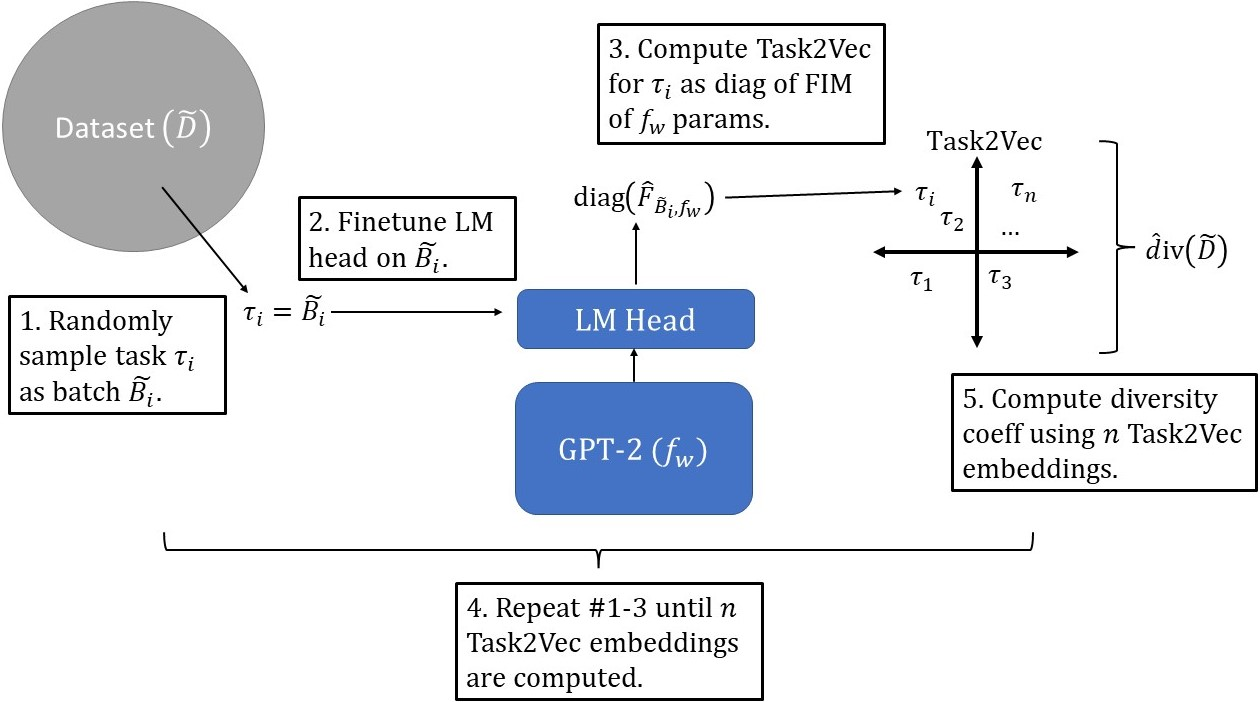
\includegraphics[width=0.5\columnwidth]{plots/diversity_project_figure_spreadout_cropped.jpg}
  \caption{
  \textbf{The process of computing the diversity coefficient for a dataset proceeds through three main stages:} (a) randomly sampling batches of text from the dataset, (b) computing the Task2Vec embeddings for each sampled batch, and (c) calculating the expected pairwise cosine distance between the Task2Vec embeddings of the sampled data.
  }
  % The first five violins show distributions of pairs of batches from the same dataset. The remaining violins show distance distributions between pairs where no two batches in a pair are from the same dataset. 
  \label{fig:div_pipeline}
\end{figure*}

Our aim is to formalize the concept of data diversity and empirically demonstrate, through \textit{interventional} experiments, its positive relationship with the evaluation performance of the validation set.  
We estimate the diversity of a dataset through the Task2Vec diversity coefficient for natural language, which embeds randomly sampled batches of data using Task2Vec embeddings \citep{task2vec} and computes the expected cosine distance between these (see Figure \ref{fig:div_pipeline}). 
It approximates the diversity of the dataset because distances between Task2Vec embeddings approximate the distance between the generative (task) distributions of the batches. 
% To compute the diversity coefficient for a given dataset, we first randomly sample batches of text sequences from a given dataset, compute Task2Vec embeddings for each of these batches, and then finally compute the expected cosine distance between these embeddings to get the value of the diversity coefficient (see Figure \ref{fig:div_pipeline}). 
% As we detail below, Task2Vec embeddings act as effective ``fingerprints" for the information that a given parameter contains for generating a batch of text \citep{task2vec, curse_low_div}. 
% Thus, by measuring the level of variation in randomly sampled embeddings, we develop an accurate and effective quantitative estimate of the diversity of data.

\subsection{Computing Task2Vec Embeddings For Text}
\label{body:computing_task2vec}
Task2Vec embeddings are defined as the diagonal of an (approximated) Fischer Information Matrix (FIM); the FIM is derived from the parameters of a fixed probe network---in the case of text data, a language model---whose final layer has been fine-tuned on the target data to embed \citep{task2vec}. 
Since the FIM encodes information on which parameters of the probe network are most important in predicting the text sequence, the diagonal of the FIM encodes a compact and tractable representation of these parameters. 
Thus, the Task2Vec embedding of text data represents which parameters of the probe network are most important in \textit{solving} the next token prediction task given by a text sequence. 
We use a probe network with final layer fine-tuning on the target data in calculating the FIM as this is the only validated method (to our knowledge) for creating Task2Vec embeddings \citep{task2vec}. 
Importantly, the probe network is fixed for all batches in order to make embeddings comparable between tasks \citep{task2vec}.

Though Task2Vec embeddings are primarily used in visual and meta-learning tasks \citep{task2vec, curse_low_div, 9577374}, we adapt and repurpose this technique to the novel domain of natural language data. 
In particular, we use GPT-2 \citep{gpt2} as our fixed probe network and fine-tune its final layer with a next-token prediction objective. 
% We use a separate probe-network for each batch embedding we compute so that fine-tuning updates are \textit{not} shared between batches.

Formally, we compute the FIM as:
\begin{equation*}
\begin{aligned}
    \hat F_B = 
        % \mathbb E_{x} 
            % \mathbb E_{t}
                \mathbb E_{x, t, \hat x_t}
                    % \nabla_w \log \hat p_w( \hat x_t \mid x_{t-1:1}) \nabla_w \log \hat p_w ( \hat x_t \mid x_{t-1:1})^\top
                    % \nabla_w log \hat p_w( \hat x_t \mid x_{t-1:1}) \nabla_w log \hat p_w ( \hat x_t \mid x_{t-1:1})^\top
                    % \nabla_w \log \hat p_w( \hat x_t \mid x_{t-1:1}) \nabla_w \log \hat p_w ( \hat x_t \mid x_{t-1:1})^\top
                    \nabla_w \log \hat p_w( \hat x_t | x_{t-1:1}) \nabla_w \log \hat p_w ( \hat x_t | x_{t-1:1})^\top
\end{aligned}
\end{equation*}
The Task2Vec embedding $\vec{f}_B$ is the diagonal of the computed FIM, i.e. $\vec{f}_B = Diag(F_B)$, where $B$ represents a batch of text sequences, $x$ is a text sequence sampled from $B$, $\hat{x}_t$ is the next token predicted by the fine-tuned probe network $f_w$ (with weights $w$) conditioned on the ground truth sequence $x_{t-1:1}$, and $t$ is a given index of the sequence.

\subsection{Computing the Diversity Coefficient for Natural Language Text}
\label{body:div_coeff_natural_lang}
The \textit{diversity coefficient} is the expected pairwise cosine distance $d$ between Task2Vec embeddings of batches of text $B_1, B_2$ sampled from a natural language dataset $D$:
\begin{equation*}
\begin{aligned}
    \hat{div}(D) =
    \mathbb{E}_{B_1, B_2 \sim D} 
     % \left[ 
     d( \vec{f}_{B_1}, \vec{f}_{B_2} )
     % \right]
\end{aligned}
\end{equation*}
By measuring the distance between Task2Vec embeddings of sampled text batches, the diversity coefficient captures the average intrinsic variability of the sampled batches, serving as an efficient estimate for the diversity of information contained in the dataset. 
It is an effective ``soft" count of the number of distinct batches. 

A useful variation on the concept of the diversity coefficient is the \textit{cross diversity coefficient}, which calculates the informational variation i.e. diversity \textit{between} \textit{separate} datasets. 
Following the framework of the diversity coefficient, the cross diversity coefficient is the expected pairwise cosine distance $d$ between Task2Vec embeddings of batches of text $B_1$ sampled from a natural language dataset $D_1$ and batches of text $B_2$ sampled from a separate dataset $D_2$:
\begin{equation*}
\begin{aligned}
    \hat{cdiv}(D_1, D_2) =
    \mathbb{E}_{B_1 \sim D_1, B_2 \sim D_2} 
     % \left[ 
     d( \vec{f}_{B_1}, \vec{f}_{B_2} )
     % \right]
\end{aligned}
\end{equation*}
We introduce these two definitions (diversity and cross diversity) to show our results hold with respect to two intuitive and logical ways to define data diversity (details in Appendix \ref{appendix:cross_div_justification}).
In addition, the \textit{cross diversity} coefficient also measures the similarity/alignment or difference \textit{between} datasets (using Task2Vec representations of data).
% such as when deciding which subcorpora to include in a large, diverse natural language corpus \citep{thepile}.

% \section{Methods}\label{methods}
% \subsection{Task2Vec Embeddings for Sequence Data} 
% We use the Task2Vec diversity coefficient \citep{curse_low_div} to compute the formal diversity of a dataset, echoing the approach of \citep{nguyen2019understanding} in using Task2Vec to characterize data. We choose Task2Vec embeddings since they have been shown to be effective ``informational fingerprints" of embedded data by, at a high level, identifying which model weights are important in performing prediction on a given batch of text sequences \citep{task2vec} (see Appendix \ref{appendix:intuitiontask2vec} for further explanation).
% The first step is to compute Task2Vec (vectorial) embeddings of a batch of sequences.
% %and explain our extensions using LLMs. 
% The original Task2Vec method \citep{task2vec} embeds data (e.g. few-shot learning task) using the diagonal entries of the Fisher Information Matrix (FIM) that result from (partially) fine-tuning the final layer of a fixed neural network (also called a \textit{probe network}) to solve the current task (or batch), similar in nature to \citep{edwards2017neural} with probe-network based data analysis.
% We implement this framework by fine-tuning GPT-2 \cite{gpt2} to predict the next token for each sequence in the current batch $B$, then compute the FIM as follows:
% \begin{equation*}
% \begin{aligned}
%     \hat F_B = 
%         % \mathbb E_{x} 
%             % \mathbb E_{t}
%                 \mathbb E_{x, t, \hat x_t}
%                     % \nabla_w \log \hat p_w( \hat x_t \mid x_{t-1:1}) \nabla_w \log \hat p_w ( \hat x_t \mid x_{t-1:1})^\top
%                     % \nabla_w log \hat p_w( \hat x_t \mid x_{t-1:1}) \nabla_w log \hat p_w ( \hat x_t \mid x_{t-1:1})^\top
%                     % \nabla_w \log \hat p_w( \hat x_t \mid x_{t-1:1}) \nabla_w \log \hat p_w ( \hat x_t \mid x_{t-1:1})^\top
%                     \nabla_w \log \hat p_w( \hat x_t | x_{t-1:1}) \nabla_w \log \hat p_w ( \hat x_t | x_{t-1:1})^\top
% \end{aligned}
% \end{equation*}
% The Task2Vec embedding $\vec{f}_B$ is the diagonal ($Diag$) of the FIM $\vec{f}_B = Diag(F_B)$, 
% % \begin{equation*}
% % \begin{aligned}
% %     \vec{f}_B = Diag(F_B)
% % \end{aligned}
% % \end{equation*}
% where $x$ is a sequence of length $T_x$ sampled from a batch $B$ i.e. $x \in B$,
% $\hat x$ is a sequence of tokens sampled from the fine-tuned probe network $f_w$ (with weights $w$) conditioned on the real sequence $x$ i.e. $\hat x \sim \hat p_{w}( \hat x_t \mid x_{t-1:1})$, 
% % $\mathbb E_{t}$ indicates taking the average across the sequence length when computing the loss.
% $t$ indicates taking the average log loss over the sequence length.
% \subsection{Diversity Coefficient Computation for Natural Language Datasets}
% \label{body:div_coeff_natural_lang}
% \subsubsection{Definition of the Diversity Coefficient}\label{div_coeff}
% Using our extension of Task2Vec for sequence data, we explain how to compute the Task2Vec diversity coefficient \citep{curse_low_div} for natural language datasets using GPT-2 as a probe network.
% %The previous formulation of the Task2Vec diversity coefficient was computed over batches of data that aligned with the specific task or sub-dataset label they were sampled from. 
% %Since this information is not always present, we propose to sample batches of data directly from the dataset.
% %Therefore, 
% We compute the Task2Vec diversity coefficient as the expected cosine distance $d$ between pairs of Task2Vec embeddings of batches:
% \begin{equation*}
% \begin{aligned}
%     \textrm{$\hat{d}$iv}(D) =
%     \mathbb{E}_{B_1, B_2 \sim D} 
%      % \left[ 
%      d( \vec{f}_{B_1}, \vec{f}_{B_2} )
%      % \right]
% \end{aligned}
% \end{equation*}
% where $D$ is the natural language dataset from which we sample batches $B_1, B_2$, and
% $\vec{f}_{B_i}$ is the Task2Vec embedding of a batch $B_i$ using the diagonal of the FIM matrix $\hat F_{B_i}$.
% In this setting, if $D$ is a \textit{union} of datasets (also known as \textit{interleaved}), then a batch contains sequences from both datasets according to some specified data mixture.

% By measuring the distance between FIMs, the diversity coefficient captures the average intrinsic variability of batches in the underlying data distribution as a proxy for data coverage or information contained in the dataset. 
% %[TO-DO: fig, appendix]
% Another interpretation is that dataset diversity reflects how different batches are from each other. See Figure \ref{fig:pipeline} in Appendix \ref{appendix:pipeline} for an illustration of this process.
% %Therefore, a low diversity coefficient implies that batches are not very different.
% \subsubsection{Definition of the Cross Diversity Coefficient}\label{cross_div_coeff}
% The cross diversity coefficient computes the expected cosine distances of (Task2Vec) embeddings of batches by sampling each batch of sequences from only one of the two datasets, without any interleaving or mixing of the sequences between datasets. 
% In other words, each batch will only contain sequences from \textit{one} of the sub-datasets, not both: 
% \begin{equation*}
% \begin{aligned}
%     \textrm{$\hat{d}$iv}(D_1, D_2) =
%     \mathbb{E}_{B_1 \sim D_1, B_2 \sim D_2} 
%      % \left[ 
%      d( \vec{f}_{B_1}, \vec{f}_{B_2} )
%      % \right]
% \end{aligned}
% \end{equation*}
% In this work, we use the term \textit{concatenated} when the sequences in each batch come only from a single data set. 
% We introduce these two definitions (diversity and cross diversity) to show our results hold with respect to two intuitive and logical ways to define data diversity (details in Appendix \ref{appendix:cross_div_justification}).


%%%%%%%%%%%%%%
\begin{table*}[t]
% 4.23 for Pile-CC
\caption{\textbf{Diversity coefficients of LLM pre-training datasets are 2.7-4.76 times higher than the conceptual lower bound and more than half that of the upper bound.}
\textbf{Cross diversity coefficients of LLM pre-training datasets are 3-5 times higher than the conceptual lower bound and more than half that of the upper bound.
Overall, any strategy of concatenating datasets increases the cross diversity coefficient}.
For the diversity coefficient, batches of text sequences were sampled from a mixed (i.e. interleaved) pool of sequences from all sub-datasets. Thus, sequences from both sub-datasets are present in the same batch at a rate dictated by the data mixture.
Mix1 stands for a data mixture with ratio 3:1 (i.e., 0.75 to 0.25) for the corresponding combined data sets.
Mix2 stands for a data mixture according to LLaMA v1 (i.e., 0.77, 0.23) for the corresponding combined data sets (see Appendix \ref{appendix:mixdetails} for details).
Note, cross diversity does \textit{not} mix datasets when computing the corresponding coefficient. Instead, we sample batches entirely from one of the sub-datasets; the distance between batches is then used to compute the cross diversity (see Appendix \ref{appendix:cross_div_justification} for explanation).
}
\vskip 0.15in
\begin{center}
\begin{small}
\begin{sc}
\begin{tabular}{lccccr}
\toprule
Dataset & Diversity Coeff. & Cross Diversity Coeff. \\
\midrule
Lower Bound (LB) & $\textbf{0.0525}\pm 3.41\textrm{e-}4$ & (same as left) \\

NIH ExPorter & $0.15 \pm 3.218\textrm{e-}5$ & (same as left)\\
USPTO & $0.1582 \pm 4.09\textrm{e-}5$ & (same as left) \\
PubMed Abstracts & $0.168 \pm 2.63\textrm{e-}5$ & (same as left) \\
HackerNews & $0.201 \pm 4.52\textrm{e-}5$ & (same as left) \\

WikiText-103 & $0.2140 \pm 7.93\textrm{e-}5$ & (same as left) \\

Combination of five datasets (Mix2) & $ \textbf{0.217} \pm 9.81\textrm{e-}4$ & $\textbf{0.2939} \pm 2.03\textrm{e-}4$ \\

SlimPajama & $0.221 \pm 9.97\textrm{e-}4$ & (same as left) \\ % https://wandb.ai/brando/beyond-scale/runs/oyspg0r9?workspace=user-brando
OpenWebtext & $ 0.222 \pm  1.00\textrm{e-}3 $ & (same as left) \\ % https://wandb.ai/brando/beyond-scale/reports/Skylion007-openwebtext-div_coeff-for-samuya--Vmlldzo1MjY0NDcw

C4 and WikiText-103 (Mix1) & $ \textbf{0.235} \pm  1.04$\textrm{e-}3 & $\textbf{0.2711} \pm 3.22\textrm{e-}4$\\ % https://wandb.ai/brando/beyond-scale/runs/i29297m2/overview?workspace=user-brando
C4 & $0.2374 \pm 2.785\textrm{e-}5$ & (same as left) \\

The Pile & $0.2463 \pm 3.034\textrm{e-}5$ & (same as left) \\
Pile-CC & $\textbf{0.2497} \pm 3.41\textrm{e-}5$ & (same as left) \\

Upper Bound (UB) & $\textbf{0.4037} \pm 1.932\textrm{e-}5$ & (same as left)\\
\bottomrule
\end{tabular}
\label{tab:div}
\end{sc}
\end{small}
\end{center}
\vskip -0.1in

\end{table*}
%%%%%%%%%%%%%%

\subsection{Backbone Used to compute the Diversity Coefficient}
To compute Task2Vec embeddings, we use GPT-2 \cite{gpt2} pre-trained on the English language as the probe network $f_w$. 
Following Task2Vec \citep{task2vec}, we fine-tune only the final layer (a language modeling head) on each batch since it's the only tested method for computing Task2Vec embeddings \cite{task2vec, curse_low_div, miranda2023pretraining}, e.g. it's not known if the intuitive properties observed in \citep{task2vec} hold without fine-tuning the backbone. 
See Figure \ref{fig:div_pipeline} for a visual of the diversity coefficient computation pipeline.

\subsection{Recipe for Establishing if a Diversity Coefficient is High via the Conceptual Lower and Upper Bounds }\label{method_ub_lb}
To establish if a diversity coefficient $\hat{\textrm{div}}(D)$ of a dataset $D$ is high (or low), we use two conceptually well-motivated reference values.
We call them the lower and upper bounds of the diversity coefficient.
% We explain the conceptually motivated lower and upper bounds of the diversity coefficient. 
To understand the lower bound, consider a dataset constructed by sampling with most of the probability mass concentrated on some arbitrary token.
This is a good candidate for a dataset with minimum diversity.
To understand the upper bound, consider the other extreme: a dataset constructed by sampling any token uniformly at random given a fixed vocabulary (in our case, the GPT-2 tokenizer vocabulary) is a good candidate to create a dataset with maximum diversity.
% The conceptually motivated lower and upper bounds of the diversity coefficient were measured on synthetic datasets constructed by sampling either from a subset of or the entirety of the GPT-2 BPE tokenizer vocabulary. 
% Intuitively, a low or no diversity dataset would consist of sequences composed from only one token, plus the \texttt{<eos>} token.

Therefore, we measure a conceptual lower bound on a dataset with a vocabulary size of $2$: \texttt{<eos>} token and a randomly selected non-special token from the GPT-2 tokenizer vocabulary. 
The \texttt{<eos>} token was assigned a probability weight of $1/\{\text{GPT-2 vocab size}\}$. 
The non-special token was assigned the remaining weight.
Similarly, a high or maximum diversity dataset would consist of random sequences of all possible tokens, with no underlying order to semantics, formatting, etc. 
The upper bound of the diversity coefficient was therefore measured on a synthetic dataset with an equal probability of occurrence assigned to all tokens in the GPT-2 tokenizer vocabulary.


%%%%%%%%%%%%%%%%%%%%%%%%%%%%%%%%%%%%%%%%%%%%%%%%%%%%%%%%%%%%%%%%%%%%%%%%%%%%%%%%%%%%%%%%
